\documentclass{article}
\usepackage[%
    left=0.5in,%
    right=0.5in,%
    top=0.5in,%
    bottom=0.5in,%
]{geometry}%
\usepackage{minitoc}
\usepackage{multicol}
\usepackage{graphicx}
\usepackage{fixltx2e}
\usepackage{hyperref}
\usepackage{hyperref}
    \hypersetup{ colorlinks = true, linkcolor = blue }
\usepackage{blindtext}

\graphicspath{ {./} }

\newcommand{\inlinecode}[2]{\colorbox{lightgray}{\lstinline
[language=#1]$#2$}}
\newcommand{\worddef}[1]{\hyperref[sec:reference]{\textit{#1}}}

\begin{document}

\section{File access}
\begin{flushleft}
Files will be composed of a number of blocks. Files are \textbf{sequential} or \textbf{random} access. Random access is essential for example in \textbf{database systems}.
\end{flushleft}

\section{Contiguous allocation}
\begin{flushleft}
\textbf{Contiguous} file systems are similar to \textit{dynamic partitioning} in memory allocation:
\begin{itemize}
	\item Each file is stored in a \textbf{single group} of adjacent blocks on the hard disk E.g. 1KB blocks, 100KB file, we need 100 contiguous blocks
	\item Allocation of free space can be done using \textbf{first fit, best fit, next fit, etc}.
\end{itemize}
\end{flushleft}

\subsection{Advantages}
\begin{itemize}
	\item \textbf{Simple to implement}: only location of the first block and the length of the file must be stored (in the directory entry)
	\item \textbf{Optimal read/write performance}: blocks are co-located/clustered in nearby/adjacent sectors, hence the seek time is minimised (remember the example in lecture on disks!)
\end{itemize}

\subsection{Disatvantages}
\begin{flushleft}
\begin{itemize}
	\item The exact size of a file (process) is not always known beforehand: what if the file size exceeds the initially allocated disk space
	\item Allocation algorithms needed to decide which free blocks to \textbf{allocate} to a given file (e.g., first fit, best fit, etc.)
	\item Deleting a file results in \worddef{external fragmentation}: de-fragmentation must be carried out regularly (and is slower than for memory)
\end{itemize}
	Contiguous allocation is still in use: CD-ROMS/DVDs External fragmentation is less of an issue here since they are write once only
\end{flushleft}

\section{Linked list allocation}
\begin{flushleft}
To avoid \textit{external fragmentation}, files are stored in separate blocks (similar to paging) that are \textbf{linked} to one another. Only the \textbf{address} of the first block has to be stored to locate a file. Each block contains a \textbf{data pointer} to the next block (which takes up space)
\end{flushleft}

\subsection{Advantages}
\begin{itemize}
	\item \textbf{Easy to maintain}: only the first block (address) has to be maintained in the directory entry
	\item File sizes can grow \textbf{dynamically} (i.e. file size does not have to be known beforehand): new blocks/sectors can be added to the end of the file
	\item Similar to paging for memory, \textbf{every} possible block/sector of disk space can be used: i.e., there is no external fragmentation!
	\item Sequential access is straightforward, although more seek operations/disk access may be required
\end{itemize}

\subsection{Disadvantages}
\begin{itemize}
	\item Random access is \textbf{very slow}, to retrieve a block in the middle, one has to walk through the list from the start
	\item There is \textbf{some} internal fragmentation; on average the last half of the block is left unused
	\item \textbf{Internal fragmentation} will reduce for smaller block sizes
	\item May result in \textbf{random disk access}, which is very \textbf{slow} (remember the example in lecture on disks)
	\item Larger blocks (containing multiple sectors) will be \textbf{faster}
	\item Space is lost within the blocks due to the pointer, the data in a block is no longer a power of 2!
	\item \textbf{Diminished reliability}: if one block is corrupt/lost, access to the rest of the file is lost
\end{itemize}

\section{File allocation tables}
\begin{flushleft}
Advantages: 
\begin{itemize}
	\item Block size remains power of 2, i.e., no space is lost due to the pointer
	\item Index table can be kept in memory allowing \textbf{fast} non-sequential/random access (one still has to walk through the table though) 
\end{itemize}
Disadvantages:
\begin{itemize}
	\item The size of the file allocation table grows with the number of blocks, and hence the size of the disk
	\item For a 200GB disk, with a 1KB block size, 200 million entries are required.
	\item Assuming that each entry at the table occupies 4 bytes, this requires 800MB of main memory!
\end{itemize}
\end{flushleft}

\section{I-nodes}
\begin{flushleft}
Each file has a small data structure (on disk) called \textbf{I-node} (index-node) that contains its attributes and block pointers. 
\begin{itemize}
	\item In contrast to FAT, an I-node is \textbf{only loaded} when the file is open (stored in system wide open file table)
	\item If every I-node consists of n bytes, and at most k files can be open at any point in time, at most n×k bytes of main memory are required 
\end{itemize}
I-nodes are composed of \textbf{direct block pointers} (usually 10), \textbf{indirect block pointers}, or a combination thereof (e.g., similar to multi-level page tables)
\end{flushleft}
\begin{center}
	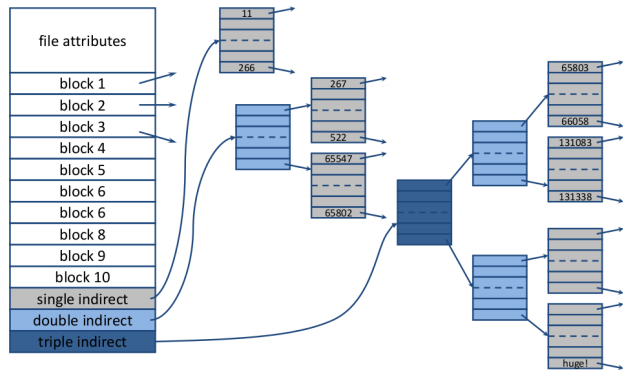
\includegraphics[scale=0.4]{i_nodes.png}
\end{center}

\subsection{Directories}
\begin{itemize}
	\item In UNIX, all information about the file (type, size, date, owner, and block pointers) is stored in its i-node. 
	\item Therefore, directory tables are very simple data structures composed of file name and a pointer to the i-node. 
	\item Note that directories are no more than a special kind of file, so they have their own i-node.
\end{itemize}

\subsection{Lookups}
\begin{flushleft}
\textbf{Opening a file} requires the disk blocks to be located. Absolute file names are located relative to the \textbf{root} directory. Relative file names are located based on the \textbf{current working directory}.\\
\enskip

Locate the root directory of the file system\\
- Its i-node sits on a fixed location at the disk
(the directory itself can sit anywhere)\\
Locate the directory entries specified in the path:\\
- Locate the i-node number for the first component
(directory) of the path that is provided\\
- Use the i-node number to index the i-node table\\
and retrieve the directory file\\
- Look up the remaining path directories by\\
repeating the two steps above\\
Once the file’s directories have been located, locate
the file’s i-node and cache it into memory
\end{flushleft}

\subsection{Sharing files}
\begin{flushleft}
There are two approaches to \textbf{share a file}, e.g. between directory B and C, where C is the ’real’ owner:
\begin{itemize}
	\item \textbf{Hard links}: maintain two (or multiple) \textbf{references to the same i-node} in B and C. (In Unix: ln /C/file1 /B/file2) the i-node link reference counter will be set to 2
	\item \textbf{Symbolic links}: The \textbf{owner maintains a reference} to the i-node in, e.g., directory C The “referencer” maintains \textbf{a small file} (that has its own i-node) that contains the location and name of the shared file in directory C. (In Unix: ln -s /C/file1 /B/file2)
\end{itemize}
\end{flushleft}

\subsubsection{Hard links}
\begin{flushleft}
Hard links are the \textbf{fastest way} of linking files! Disadvantages of hard links:
\begin{itemize}
	\item Assume that the \textbf{owner} of the file \textbf{deletes} it: If the i-node is also deleted, any hard link will, in the best case, \textbf{point to an invalid i-node}. If the i-node gets deleted and “recycled” to point to an other file, the hard links will point to the \textbf{wrong file}!
	\item The only solution is to delete the file, and \textbf{leave} the i-node intact if the “reference count” is \textbf{larger than 0} (the original owner of the file still gets “charged” for the space)
\end{itemize}
\end{flushleft}

\subsubsection{Soft links}
\begin{flushleft}
Disadvantages of soft links:
\begin{itemize}
	\item They result in an \textbf{extra file lookup} (once the link file has been found, the original file needs to be found as well)
	\item They require an \textbf{extra i-node} for the link file
\end{itemize}
Advantages of symbolic links:
\begin{itemize}
	\item There are \textbf{no problems} with deleting the original file, then the file simply does not exist any more
	\item They can \textbf{cross the boundaries} of machines, i.e. the linked file can be located on a different machine
\end{itemize}
\end{flushleft}

\pagebreak
\section*{Reference section} \label{sec:reference}
\begin{description}
	\item[external fragmentation] \hfill \\ External fragmentation is the various free spaced holes that are generated in either your memory or disk space.
\end{description}
\end{document}
